\chapter{The RoFI platform}\label{chap:rofi}

The goal of the RoFI platform is to create a new platform for distributed,
modular and self-reconfigurable robots. The platform does not target real-world
usage but it should serve as a tool for validation of various control algorithms
in a physical world. This chapter presents the platform and gives an in-depth
specification of it.

First, we give a brief introduction to a concept of modular robots and establish
several terms. Then we specify the goals of the RoFI platform and provide its
specification. The specification is given as it is without any reasoning behind
the design choices. The reasoning can be found in the following chapter
\ref{chap:behind}.

\section{Modular Robots}

An modular robotic platform is a way to build robots consisting of
\emph{modules}, as the name suggests. For our purposes, we consider a module to
be a single unit following a specification given by the platform. Modules are
rather high-level pieces with a certain level of self control instead of
low-level components like individual actuators or sensors. It might even make
sense to talk about modules as individual robots, which are used to build other
robots\cite{brunete_current_2017}.

Each of these modules has a given set of capabilities. By joining multiple
modules and via their cooperation, new capabilities can emerge. Different
configurations of modules can emerge different capabilities. The modules are
usually mechanically connected together to form a single robot.

The mechanical connection of the modules can be done externally, e.g. by an
operator, or can be performed by the modules on each own. In the later case, we
talk about \emph{self-reconfigurable} modules \cite{brunete_current_2017}.
Depending on the topology of the connection, there is a naming established in
the literature\cite{brunete_current_2017}:
\begin{enumerate*}
    \item \emph{chain type} for a linear, snake-like and tree-like configurations,
    \item \emph{lattice type} for an regular grid-based robots,
    \item \emph{hybrid type} for robots combining both previous approaches.
\end{enumerate*}
Further, if there is only a single or a few types of modules in the system, it
is called \emph{metamorphic}\cite{brunete_current_2017}. Modules of such system
are also called \emph{cells} as they mimic cells in living organisms.

As the robot is form, it can be either \emph{centrally controlled} by a single
(and possibly external) unit or the distributed nature of the modules can be
leveraged and therefore, the robot can feature \emph{distributed control}. The
centrally controlled approach is considered as an easier one, however it does
not utilize all the potential computational power of the modules and is harder
to make fault-tolerant in case of failure of the control unit compared to the
distributed control.

To help to build an intuition about the platform we give an analogy with
Replicators -- robots present in a sci-fi TV series Star Gate. Readers
unfamiliar with the TV series can skip the following paragraph.

Replicators consist of a single Replicator block, which is unable to perform any
action on its own. Single replicator block maps to a module in terminology given
above. However, when multiple blocks are combined, they are able to perform
movement and self-control. Therefore, Replicators are:
\begin{enumerate*}
    \item modular (they can be assembled in many configurations from a single
    type of unit)
    \item self-reconfigurable (the configuration can be changed by the blocks on
    their own) and
    \item metamorphic (as there is only a single type of block).
\end{enumerate*}
Whether Replicators are distributed is unclear -- the series does not give much
detail about it. We strongly believe so, as each blob of modules can operate
independently on the others an in case of reconfiguration all newly emerged
blobs become independent.

\section{Goals of the RoFI Platform}

The goal of the RoFI platform is to give an reasonably easy way to validate
various control algorithms for modular self-reconfigurable robots, as we
mentioned in the introduction. It does not target for any specific real-world
usage, like e.g. the Roombots\cite{bonardi_locomotion_2012} for being a smart
furniture. To fullfil these goals we give a following list of requirements for
the platform:

\begin{itemize}
    \item All sources (including CAD models, PCBs, firmwares and libraries)
    should be kept open-source, to allow for reproducibility of experiments
    performed on the platform.
    \item It should be manufacturable by a commonly accessible machinery.
    \item No deep understanding of mechanical nor electrical engineering should
    be required to use it.
    \item Clear specification of the modules should be available to allow for
    further extension. It should also contain a formal apparat to describe
    systems and reason about them.
    \item The platform should provide a way to easily distribute new firmware to
    the modules.
    \item The platform should allow for both, central and distributed control.
    \item The platform should provide an easy way to port control algorithms.
    This reduces to a requirement for an easy way to define an atomic control
    actions used by the algorithms.
\end{itemize}

\section{The RoFI Platform}

The RoFI platform is a lattice type modular, self-reconfigurable and metamorphic
platform. The platform is defined by:
\begin{enumerate}
    \item a grid system with a module shape requirements (section \ref{sec:aware}),
    \item a docking system (section \ref{sec:dock}),
    \item module descriptions (section \ref{sec:capabilities}) and
    \item an intermodule communication (section \ref{sec:communication}).
\end{enumerate}

The platform also provides a formalism for describing configurations of systems
built in the platform (section \ref{sec:configuration}) and also gives an
example of a module fulfilling the specification in form of the Universal
module (chapter \ref{chap:universal_module}).

\section{Module Shape}\label{sec:aware}

The shape of modules in the RoFI platform is based on a 10cm cube grid. There is
a inscribed sphere in each cell of the grid. By saying a module \emph{occupies a
grid cell} we mean that it occupies the sphere inscribed to the cell. Two grid
cells are adjacent if they share a common face. Therefore, each cell has 6
adjacent cells.

Each module in its default state (with all joints in neutral
position\footnote{definition of joint follows in the text}) should occupy one or
more adjacent cells of the grid. If the module occupies more than a single cell,
it is also allowed to occupy space of corresponding \emph{body hull}. Consider
two adjacent cells occupied by the body. Then there is a convex hull of their
inscribed spheres (see double cell module in figure \ref{fig:rofi_shapes}). The
body hull is then defined as union of all such existing convex hulls for the
body. See \ref{fig:rofi_shapes} for an example.

\begin{figure}
    \centering
    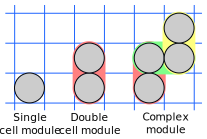
\includegraphics[width=0.7\textwidth]{figures/rofi_shapes.pdf}
    \caption{Example of a body hull construction. Each convex hull of adjacent
    cells is denoted by a coloured area. The body hull is the union of coloured
    ares. Note that the coloured areas slightly overlap the grid. This is only
    for the purpose of visualizations. In reality they fit exactly in the grid.}
    \label{fig:rofi_shapes}
\end{figure}

The modules are allowed to change their shape by featuring several degrees of
freedom in form of \emph{joints}. Joint is a rotational degrees of freedom along
given axis. We do not allow any other type of motion -- therefore e.g.
retractable nor sliding modules are not allowed in the RoFI platform.
Intuitively, we can view a module as beads, which can rotate against each other
along the axis of joints. For an simple example of a double cell module movement
see figure \ref{fig:grid_aware}.

The motivation for such a restriction of the shape is a property we call
\emph{grid-awareness}. Consider a simple task for a double cell module: having a
grounded left part of the module, move its right part above the left one. This
task is illustrated in figure \ref{fig:grid_aware}. If we consider a module
which fits exactly inside a cube-shaped cell, e.g. an M-TRAN module
\cite{haruhisa_kurokawa_m-tran_2003}, the module occupies extra cells during the
movement (marked by red circles in the figure). This restricts the module
movement in a densely occupied grids. However, if we consider a grid-aware
module (in the example double cell module), it only occupies the least required
cells for the movement and therefore should allow for more efficient
reconfiguration algorithms. Grid-awareness however comes at a const. It requires
a retractable docking mechanism as two neighbouring modules can feature only a
point contact. We further discuss this in section \ref{sec:dock}.

\begin{figure}
    \centering
    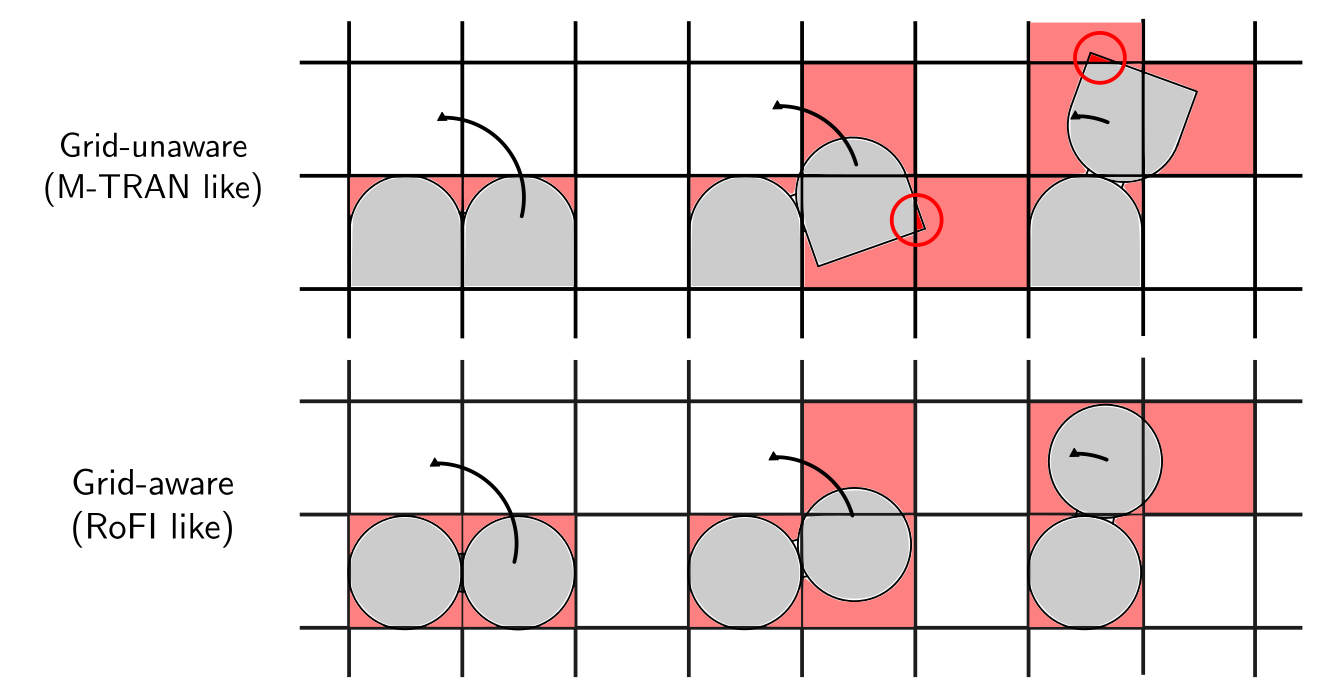
\includegraphics[width=\textwidth]{figures/grid_aware.pdf}
    \caption{Visualization of grid-awareness. Consider two module shapes -- an
    M-TRAN\cite{haruhisa_kurokawa_m-tran_2003} like (int the top row) and a RoFI
    like (in the bottom row). Given the task to move right body over the left
    one, M-TRAN like module occupies extra cells due to small parts of it body
    overlapping out of the gird. On the other hand, RoFI like module occupies
    the least cells required to make the movement. }
    \label{fig:grid_aware}
\end{figure}

We would like to point out that even we referred all examples to a grid-fitting
positions of the robots (where all movement is performed by steps of
$90^\circ$), we do not give any restriction on the granularity of the movement.
We assume the modules are physically able to perform practically unlimited
granularity (considering limits of a mechanic construction). However, the
reconfiguration algorithms built on top of the system can consider only a
discrete steps in the movement if they need to.

The shape specification allows us to define modules with various shape and
functionality. However, we do not expect the platform to feature many different
types of modules and especially oddly shaped ones. We strongly believe that a
double cell module, called \emph{universal module} (described in chapter
\ref{chap:universal_module}), should be the main building block of RoFI systems.
However, in future we consider having e.g.
\begin{itemize}
    \item a passive module (only a mechanical construction),
    \item battery module or
    \item single-cell modules featuring specialized sensors (e.g. camera) or
    actuators (e.g. robotic hand or a wheel).
\end{itemize}


\section{RoFI Docking System}\label{sec:dock}

Being the modules in the RoFI platform grid-aware, we cannot easily adapt
existing docking systems from systems like
Roombots\cite{bonardi_locomotion_2012} or MTRAN III
\cite{kurokawa_distributed_2008}. The reason for that is two adjacent modules in
the grid feature only a single point contact and not a whole face contact as it
is common in other modular robotic platforms. There is a need for a retractable
docking system (see \ref{fig:rofi_locking_example}).

\begin{figure}
    \centering
    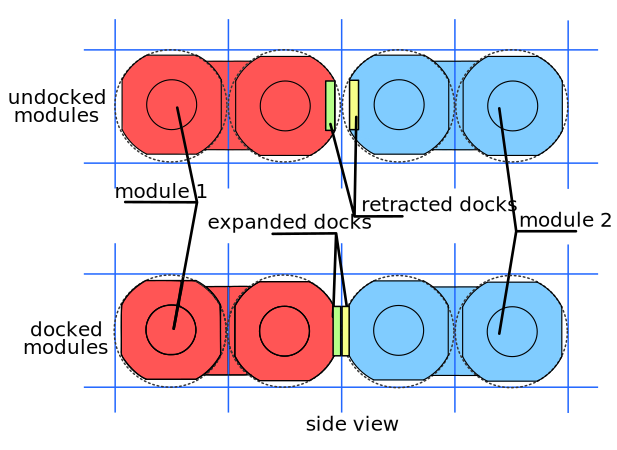
\includegraphics[width=\textwidth]{figures/rofi_locking_example.pdf}
    \caption{Docking procedure. There is a by-default retracted docking system
    in the module which expands when the docking should be performed.}
    \label{fig:rofi_locking_example}
\end{figure}


\begin{figure}
    \centering
    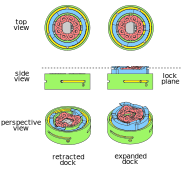
\includegraphics[width=\textwidth]{figures/dock_overview.pdf}
    \caption{The dock from the RoFI docking system. The model is simplified.}
    \label{fig:dock_overview}
\end{figure}

To overcome this issue, we present the RoFI docking system (figure
\ref{fig:dock_overview}). This docking system is inspired by the HiGen docking
system \cite{parrott_higen:_2014}. In summary, our docking system:
\begin{itemize}
    \item allows for connection of two modules when they are not touching side
    by side,
    \item is genderless (each two docks can connect),
    \item it is based on a mechanical connection (and therefore is not limited
    by a magnetic force),
    \item allows for disconnection without participation of the mating side,
    \item supports communication and power sharing and
    \item is more compact compared to the HiGen dock.
\end{itemize}

The docking system is designed to become a stand-alone unit with given
interface, which can be possibly mass produced and reused in all modules.

\subsection{The Principle of Operation}

The main principle of operation is the same as the principle of the HiGen dock.
There are two key components -- clip and skirt (figure
\ref{fig:dock_key_components}). The clip features four latches which can be
slide under latches of the clip from mating side and form a connection which
prevents pulling the docks apart. When two skirts touch each other they prevent
the two mating docks from rotating against each other. By combining these two
types of joints, we obtain a firm connection between the two docks.

The operation of a single lock is straightforward -- see figures
\ref{fig:dock_overview} and \ref{fig:dock_description}. Consider a dock in
the retracted position. When shaft ring (yellow) starts to rotate, it translates
the motion to the clip (blue). There is a helical slot in the dock body (green)
which forces the clip to move upwards (to "unscrew"). As the clip moves upwards
it carries the skirt. The skirt moves in a slot which prevents it from rotating
against body and therefore it only moves upwards. So far, the clip is extended
to a locking distance, however the latches of the docks could not slide under
each other. The end of the slot in the body is not helical and is straight (see
\todo{figure of the body}). This allows for sliding the latches under each
other.

\begin{figure}
    \centering
    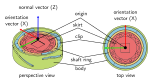
\includegraphics[width=\textwidth]{figures/dock_description.pdf}
    \caption{Naming of the components of the dock. The orientation and the
    normal vector are important for specifying orientation of two connected
    docks. }
    \label{fig:dock_description}
\end{figure}

\begin{figure}
    \centering
    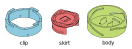
\includegraphics[width=0.75\textwidth]{figures/dock_key_components.pdf}
    \caption{View of three key components of the dock: clip, skirt and the
    middle part of the body.}
    \label{fig:dock_key_components}
\end{figure}

See figure \ref{fig:dock_locking_process} for an example of an interaction of
two docks. Situation 1 shows the docks in a position they are in two adjacent
grid cells. By rotation of the shaft ring the clips and skirts extends
(Situation 2). Situation 3 show fully expended clips and skirts. The skirts are
now connected and no rotation movement of the docks is possible. The clips are
also in the end of the helical slot. By further rotation of the shaft ring the
clips slides under each other and finish the locking process (situation 4).

\begin{figure}
    \centering
    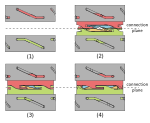
\includegraphics[width=\textwidth]{figures/locking_process.pdf}
    \caption{\todo{dock locking}}
    \label{fig:dock_locking_process}
\end{figure}

There are two important observation to note:
\begin{enumerate*}
    \item the docks are symmetric, therefore there are 4 different orientation
    the docks can lock in;
    \item the movement of two docks does not have to be synchronized and
    therefore, it is possible for a dock to wait in expanded position or to
    disconnect when the mating module stops responding.
\end{enumerate*}

The symmetry of the dock is best to shown on the skirt -- see figure
\ref{fig:dock_skirt_symmetry}. The skirt is divided into four identical blocks
along the horizontal and vertical axis. This allows for four different
orientation of the docks. When two skirts are facing there is a mapping of
blocks from one skirt to the other one. The facing blocks have the property that
the green circle is always facing a red one. This feature is is important for
three reasons:
\begin{itemize}
    \item It allows to build pins, which prevents the skirts from rotation (see
    perspective view in figure \ref{fig:dock_key_components}).
    \item Also by placing magnets in the holes (red -- north facing up, green --
    south facing down) the skirts attract to each other. This helps misaligned
    docks to connect properly.
    \item By mounting pogo pins \todo{cite} in the symmetry blocks we can build
    power and data transmission lines between modules.
\end{itemize}
There is the same idea behind symmetry of the clip as the idea behind the skirt
symmetry.

\begin{figure}
    \centering
    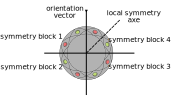
\includegraphics[width=0.8\textwidth]{figures/skirt_symmetry.pdf}
    \caption{Illustration of the skirt symmetry.}
    \label{fig:dock_skirt_symmetry}
\end{figure}

\subsection{Dock Implementation}

The dock outside diameter is

\begin{figure}
    \centering
    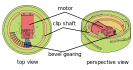
\includegraphics[width=\textwidth]{figures/dock_arrangement.pdf}
    \caption{Internal arrangement of the components inside the dock. Note that
    skirt and clip are not shown.}
    \label{fig:dock_internal_arrangement}
\end{figure}

\subsection{Dock Connectors and Communication}

\todo{Finish it!}
\todo{Docks exchange data using serial line}

\subsection{Mutual Orientation of the Docks}\label{sec:mutual_orientation}

To be able to describe system made out of modules in the section
\ref{sec:configuration} we define \emph{mutual orientation} of the docks. As
shown in figure \ref{fig:dock_description}, there is an orientation vector on
the dock. When two docks connect, there can be an angle of $0^\circ$,
$90^\circ$, $180^\circ$ or $270^\circ$ between their orientation vectors
(measured counter clockwise from a perspective one of the modules from shoe
center to the dock center). Notice, that the angle is the same no matter which
module we choose. Therefore, we give a following convention for the mutual
orientation:

If we aim one of the orientation vectors up (to the \emph{north}), the other
vector aims either:
\begin{enumerate*}
    \item \emph{north},
    \item \emph{east},
    \item \emph{south} or
    \item \emph{west}
\end{enumerate*}
as shown on figure \ref{fig:dock_orientation}. Therefore we define the mutual
orientation $o$ to be an element of $\mathcal{O} = \{N, E, S, W\}$.

\begin{figure}
    \centering
    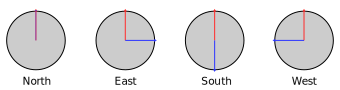
\includegraphics[width=\textwidth]{figures/dock_orientation.pdf}
    \caption{Possible orientation of two docks. Orientation vector of current
    perspective is shown as red, the orientation vector of mating dock is shown
    as blue. Note that during a connection, it does not matter which dock's
    perspective we choose.}
    \label{fig:dock_orientation}
\end{figure}


\subsection{Docks in the Grid System}

\begin{figure}
    \centering
    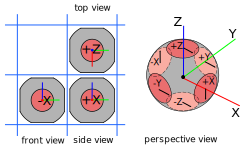
\includegraphics[width=\textwidth]{figures/dock_positions.pdf}
    \caption{Given a cell sphere the docks are allowed on 6 positions -- in the
    middles of faces of the corresponding cell cube. The docks are named using
    the axis names. Small arrows denote orientation vector of each dock. The
    vectors follow orientation of previous axe (e.g. dock +Z has an orientation
    vector in direction of the Y axe).  }
    \label{fig:dock_positions}
\end{figure}

\todo{symmetry}
\todo{comparison to HiGEN}
\todo{internal arrangement}
\todo{dimensions}
\todo{Connectors}
\todo{Manufacturing detail}
\todo{Model}
\todo{Placement on the module}

\section{RoFI Capabilities}\label{sec:capabilities}

The section \ref{sec:aware} gives an idea about all possible shapes the RoFI
modules can feature and also provides examples of use cases for shape other than
the universal module. To allow an interaction of different modules and also to
build a formal description of RoFI systems, there is a need to establish a way
to describe various modules and their capabilities.

\todo{Give a proper example}


\section{RoFI Configurations} \label{sec:configuration}

To ease and unify the development of a firmware and reconfiguration algorithms,
we give means to describe the system consisting out of RoFI modules. First,
there is a globally unique ID (\emph{GUID}) assigned to each module. GUID is a
128-bit number. Second, when talking about RoFI systems, we distinguish two
terms: \emph{topology} and \emph{configuration}:

\paragraph{topology} Intuitively, topology describes the connection between the
modules in a system and does not care about physical layout of the modules.
Formally, we define it as an undirected graph, where:
\begin{itemize}
    \item nodes are labeled by module GUIDs. There is exactly one node for each
    module in the system.
    \item edges represent a connection of two docks. The edge is labeled by a
    pair describing the connection. For modules with GUIDs $a$ and $b$,
    connection by docks $d_a$ and $d_b$ in an orientation $o$ the label is: $(o,
    \{(a, d_a), (b, d_b)\})$. There is at most one edge for each dock on the
    module. The orientation of docks is defined further in the text. Note that
    undirected edges enforces that both modules has to actively participate on a
    connection.
\end{itemize}
\todo{Give an example (text + figure)}

\paragraph{configuration} Intuitively, configuration is a topology with the
actual module positions. Formally, it is a pair $(G, L)$, where $G$ is a
topology and $L: \text{GUID} \rightarrow \text{Axis} \rightarrow \mathcal{R}$ is
a function giving us position of each axis of each module.

We define a \emph{model} $M = (V, D)$ of an configuration. $V$ is set of spheres
in 3D space over-approximating shape of the modules in a system. $D$ is a set of
named orientation vectors of all docks in the system positioned in space. Both
$D$ and $V$ can be computed via transformation matrixes build from axis
orientation and knowledge of module geometry.

We call a configuration $C = (G, L)$ with \emph{realizable} iff:
\begin{enumerate}
    \item no two spheres in $D$ intersects and
    \item for each two docks that are connected in $G$:
        \begin{enumerate}
            \item their orientation agrees with orientation in $L$,
            \item their origin points are the same and
            \item the plane defined by their orientation vectors is perpendicular to axis of a dock.
        \end{enumerate}
\end{enumerate}
Note, that there are no constraints on topology and we consider every topology
as valid. However, for some topologies there exists no possible configuration.
\todo{Give example of possible configuration, impossible due to both factors}

\section{Intermodule Communication}\label{sec:communication}

